\documentclass[10pt]{beamer}

% Beamer style
%\usetheme[secheader]{Madrid}
\usetheme{CambridgeUS}
\usecolortheme[rgb={0.65,0.15,0.25}]{structure}
%\usefonttheme[onlymath]{serif}
\beamertemplatenavigationsymbolsempty
%\AtBeginSubsection

% Packages
%\usepackage[french]{babel}
\usepackage[latin1]{inputenc}
\usepackage{color}
%\usepackage{dsfont, stmaryrd}
\usepackage{amsmath, amsfonts, amssymb}
\usepackage{xspace}
\usepackage{epsfig}
\usepackage{../../../../LATEX/Biblio/astats}
%\usepackage[all]{xy}
\usepackage{graphicx}

% Commands
\definecolor{darkred}{rgb}{0.65,0.15,0.25}
\definecolor{darkgreen}{rgb}{0,0.4,0}
\newcommand{\emphase}[1]{\textcolor{darkred}{#1}}
%\newcommand{\emphase}[1]{{#1}}
\newcommand{\paragraph}[1]{\textcolor{darkred}{#1}}
\newcommand{\refer}[1]{\textcolor{gray}{[\cite{#1}]}}
\newcommand{\Refer}[1]{\textcolor{gray}{[#1]}}
%\newcommand{\newblock}{}
\newcommand{\ra}{$\emphase{\rightarrow~}$}

% Symbols
\newcommand{\Bcal}{\mathcal{B}}
\newcommand{\Esp}{\mathbb{E}}
\newcommand{\Gam}{\mathcal{G}\text{am}}
\newcommand{\Hcal}{\mathcal{H}}
\newcommand{\Ncal}{\mathcal{N}}
\newcommand{\NBcal}{\Ncal\Bcal}
\newcommand{\Mcal}{\mathcal{M}}
\newcommand{\Pcal}{\mathcal{P}}
\newcommand{\Var}{\mathbb{V}}

%====================================================================
\title{Dispersion modeling for RNAseq differential analysis}

\author[S. Robin]{E. Bonafede$^1$, F. Picard$^2$, S. Robin$^3$, C. Viroli$^1$}

\institute[AgroParisTech / INRA]{
  \bigskip
  ($^1$) univ. Bologna, \quad ($^3$) CNRS/univ. Lyon I, \quad ($^3$) INRA/AgroParisTech, Paris
  \bigskip
% \begin{tabular}{ccccc}
%    
\includegraphics[width=.1\textwidth]{../FIGURES/LogoINRA-Couleur} & 
%    \hspace{.02\textwidth} &
%    
\includegraphics[width=.15\textwidth]{../FIGURES/logagroptechsolo} & 
%    \hspace{.02\textwidth} &
%    
\includegraphics[width=.1\textwidth]{../FIGURES/logo-ssb} \\ 
%  \end{tabular} \\
%  \bigskip
  }

  \date[IBC, Victoria]{IBC, Victoria, July 2016}

%====================================================================

%====================================================================
%====================================================================
\begin{document}
%====================================================================
%====================================================================

%====================================================================
\frame{\titlepage  }

%====================================================================
%====================================================================
\section{Modeling dispersion in RNAseq experiments}
\frame{\tableofcontents[currentsection]}
%====================================================================
\frame{\frametitle{General problem}
	
	\paragraph{RNAseq} is a sequencing based technology that gives access to a measure of the expression level of all the genes from a given species in a given sample (condition) 
	
	\bigskip\bigskip
	\paragraph{Differential analysis:} $p$ genes, $d$ conditions (possibly with replicates). \\~ \\
	\ra Find the genes, the expression of which vary across conditions.
	
	\bigskip\bigskip
	\paragraph{Data.}
	$$
	Y_{ijr} = \text{RNAseq read count for gene $i$ in replicate $r$ of condition $j$}
	$$	
	}

%====================================================================
\frame{\frametitle{Negative binomial model}
	
	\paragraph{RNAseq count =} number of reads mapped onto a gene's sequence. 
	\\ ~ \\
	\ra Observed variability often exceeds this expected according to Poisson. 
	
	\bigskip\bigskip\pause
	\paragraph{Popular model.} \refer{RMS10} 
	$$
	Y_{ijr} \sim \NBcal(\lambda_{ij}, \alpha_i)
	$$
	where $1/\alpha =$ over-dispersion parameter: $\Var(Y_{ijr}) = \lambda_{ij} (1 + \lambda_{ij}/\alpha_i).$
	
	\bigskip\bigskip\pause
	\paragraph{Differential analysis.} For each gene $i$, test
	$$
	H_0 = \{\lambda_{i1} = \lambda_{i2}\} 
	\qquad\text{vs}\qquad
	H_1 = \{\lambda_{i1} \neq \lambda_{i2}\} .
	$$ 	
	}

%====================================================================
\frame{\frametitle{Modeling over-dispersion}
	
	\paragraph{Assumption on $\alpha$:} 
	\begin{itemize}
	\item Same $\alpha$ for all genes: unrealistic;
	\item Gene-specific $\alpha_i$: hard to estimate, especially with few replicates.
	\end{itemize}
		
	\bigskip\bigskip\pause
	\paragraph{Several approaches:}
	\begin{itemize}
	\item Shrinkage: {\tt edgeR} \refer{RoS08,McC12}, {\tt DSS} \refer{WWW13}; \\
	\item Function of mean expression: \refer{Law15}, {\tt NBPseq} \refer{DSC11}, {\tt DEseq} \refer{AnH10,Lov14};
	\item Bayesian estimation: {\tt baySeq} \refer{HaK10};
	\item Mixture model: {\tt DEXUS} \refer{KUH13} (components = conditions)
	\end{itemize}
	
	\bigskip
	+ many others: {\tt NOISeq} \refer{TGD11}, {\tt PoissonSeq} \refer{LiT13}, {\tt QuasiSeq} \refer{LNM12},  {\tt TSPM}  \refer{AuD11} {\tt }  {\tt }

	}

%====================================================================
\frame{\frametitle{Mixture model for the dispersion}
	
%	\paragraph{Our approach:} 
%	Mixture-model for the dispersion, similar to \refer{DRD05,DRL05} for microarray expression (Gaussian setting).
	
%	\bigskip\bigskip
	\paragraph{Poisson-Gamma representation.}
	$$
	U \sim \Gam(\alpha, \alpha), \quad 
	Y \,|\, U \sim \Pcal(\lambda U) \qquad
	\Rightarrow \qquad
	Y \sim \NBcal(\lambda, \emphase{\alpha})
	$$
	\ra Over-dispersion generated by the latent variable $U$.
	
	\bigskip\bigskip\pause
	\paragraph{Mixture model for the dispersion.} Genes belong to $K$ different dispersion groups: \\~ \pause
% 	\begin{itemize}
% 	\item Dispersion group of gene $i$: \qquad $Z_i \; \sim \; \Mcal\left(1; (\omega_k)\right)$; \\~ \pause
% 	\item Latent dispersion variable: \qquad  $U_{ijr}\,|\,Z_i=k \; \sim \;  \Gam(\emphase{\alpha_k}, \emphase{\alpha_k})$; \\~ \pause
% 	\item Observed count: \qquad\qquad\qquad $Y_{ijr} \,|\, U_{ijr} \; \sim \;  \Pcal(\lambda_{ij} U_{ijr})$.
% 	\end{itemize} 
	$$
	\begin{array}{lcrcl}
	\text{Dispersion group of gene $i$:} & & Z_i & \sim & \Mcal\left(1; (\omega_k)\right); \\ \\ \pause
	\text{Latent dispersion variable:} &  &U_{ijr}\,|\,Z_i=k & \sim &  \Gam(\emphase{\alpha_k}, \emphase{\alpha_k}); \\ \\ \pause
	\text{Observed count:} & & Y_{ijr} \,|\, U_{ijr} & \sim &  \Pcal(\lambda_{ij} U_{ijr}).
	\end{array}
	$$
	
	}

%====================================================================
\frame{\frametitle{Distributions}

  \begin{tabular}{cc}
    $U_{ijr} \sim \Gam(\alpha_k, \alpha_k)$ 
    &
    \hspace{-.05\textwidth}
    $Y_{ijr} \sim \NBcal(\lambda, \alpha_k)$ \\
    \begin{tabular}{p{.45\textwidth}}
      \includegraphics[width=.45\textwidth]{../FIGURES/BPR15-Biometrics-MixtGamma}
    \end{tabular}
    &
    \hspace{-.05\textwidth}
    \begin{tabular}{p{.45\textwidth}}
    \includegraphics[width=.45\textwidth]{../FIGURES/BPR15-Biometrics-MixtNegBinom}
    \end{tabular}
  \end{tabular}
}

%====================================================================
\frame{\frametitle{Graphical representation}

  For gene $i$:
  $$
  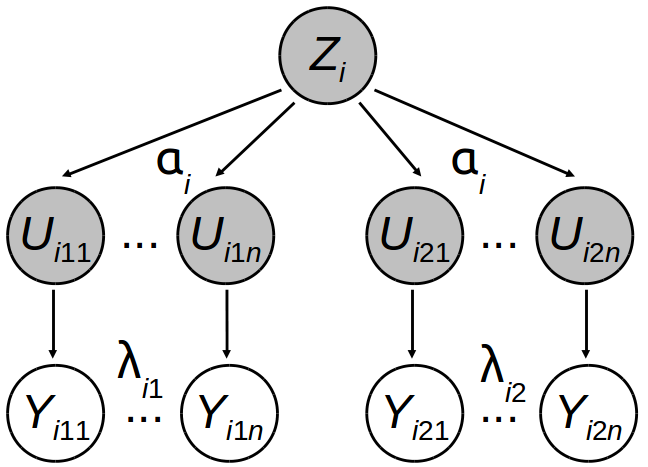
\includegraphics[width=.45\textwidth, clip=]{../FIGURES/BPR15-Biometrics-ModGraph.png}
  $$
  
  \bigskip
  \paragraph{Marginal distribution:}
  $$
  Y_{ijr} \,|\, Z_i=k \sim \NBcal(\lambda_{ij}, \alpha_k), 
  \qquad
  Y_{ijr} = \sum_k \omega_k \NBcal(\lambda_{ij}, \alpha_k)
  $$
}


%====================================================================
%====================================================================
\section{Statistical inference \& Test statistics}
\frame{\tableofcontents[currentsection]}
%====================================================================
\frame{\frametitle{A two-hidden layer model}

  \begin{itemize}
   \item Parameter $\theta = \left\{\omega = (\omega_k), \alpha = (\alpha_k), \lambda = (\lambda_{ij})\right\}$;
   \item Hidden variables $H = \left\{Z = (Z_i), U = (U_{ijr})\right\}$;
   \item Observed variables $Y = (Y_{ijr})$.
  \end{itemize}
  
  \bigskip\bigskip\pause
  \paragraph{Likelihood decomposition.} \refer{DLR77}
  \begin{eqnarray*}
   \log p_\theta(Y) & = & \log \int p_\theta(Y, H) \text{d}H \\ ~\\ \pause
    & = & \Esp \left[\log p_\theta(Y, H) \,|\, Y\right] + \Hcal\left[p_\theta(H\,|\,Y)\right] \\ ~\\ \pause
    & = & \Esp \left[\log p_\omega(Z) + \log p_\alpha(U \,|\, Z) + \log p_\lambda(Y \,|\, U) \,|\, Y\right] %\\ ~\\
    %& & 
    + \Hcal\left[p_\theta(H\,|\,Y)\right] 
  \end{eqnarray*}

}

%====================================================================
\frame{\frametitle{EM algorithm}
  
  \paragraph{Aim:} Find $\widehat{\theta} = \arg\max_\theta \log p_\theta(Y)$.
  
  \bigskip\bigskip\pause
  \paragraph{E step:} Compute conditional moments
  \begin{itemize}
   \item $Z \,|\, Y:$ multinomial;
   \item $U \,|\, Y:$ mixture of Gammas.
  \end{itemize}

  \bigskip\bigskip\pause
  \paragraph{M step:} Estimate the parameters
  \begin{itemize}
   \item $\widehat{\omega}_k:$ explicit;
   \item $\widehat{\alpha}_k:$ numerical via quasi-Newton (or fix-point);
   \item $\widehat{\lambda}_{ij}:$ explicit.
  \end{itemize}
}

%====================================================================
\frame{\frametitle{Three contrasts}

  \paragraph{Test:} 	
  $
  \qquad
  H_0 = \{\lambda_{i1} = \lambda_{i2}\} 
  \qquad\text{vs}\qquad
  H_1 = \{\lambda_{i1} \neq \lambda_{i2}\} .
  $ 	
  
  \bigskip\bigskip\pause
  \paragraph{Considered contrasts:}
  \begin{eqnarray*}
   \text{Difference} & = & \widehat{\lambda}_{i1} - \widehat{\lambda}_{i2} \\
   \text{Ratio} & = & \widehat{\lambda}_{i1} / \widehat{\lambda}_{i2} \\
   \text{Log-ratio} & = & \ln\left(\widehat{\lambda}_{i1} / \widehat{\lambda}_{i2}\right)
  \end{eqnarray*}

  \bigskip\bigskip\pause
  \paragraph{Constrast variance:} First-order approximation derived via the $\Delta$-method. 
  $$
  \text{Test statistic} = \text{Contrast} \left/ \sqrt{\Var(\text{Contrast})} \right.
  $$
  

}

%====================================================================
%====================================================================
\section{Simulations \& Illustration}
\frame{\frametitle{Outline} \tableofcontents[currentsection]}
%====================================================================
\frame{\frametitle{Simulation design}

  \paragraph{{\tt compcodeR} package \refer{Son14}:}  Independent 'realistic' RNAseq simulation.
  \begin{itemize}
   \item $p = 1000, 5000$ genes (inc. 10\% down- and 10\% up-regulated);
   \item $d = 2$ conditions;
   \item $n_j = 3, 5, 10$;
   \item Library size $= 10^6$.
  \end{itemize}
  
  \bigskip
  \paragraph{Evaluation criteria}
  \begin{itemize}
   \item Type-I error control;
   \item ROC curve
   \item Estimation of the dispersion:
   $$
   \widehat{\Var}(Y_{ijr}) = \widehat{\lambda}_{ij} \left(1 +
   \widehat{\lambda}_{ij} \sum_k \Esp_{\widehat{\theta}}(Z_{ik} \,|\, Y) /
   \widehat{\alpha}_k\right)
   $$
  \end{itemize}

}

%====================================================================
\frame{\frametitle{Type-I error control \small{($p = 1000$)}}
	
	\vspace{-.05\textheight}
	$$
	\includegraphics[height=.9\textheight]{../FIGURES/BPR15-Biometrics-Fig1}
	$$
	}

%====================================================================
\frame{\frametitle{ROC curves  \small{($p = 5000$)}}
		
	\vspace{-.05\textheight}
	$$
	\includegraphics[height=.9\textheight]{../FIGURES/BPR15-Biometrics-Fig2}
	$$
	}

%====================================================================
\frame{\frametitle{Estimation of dispersion  \small{($p = 5000$)}}
		
	\vspace{-.05\textheight}
	$$
	\begin{tabular}{p{.4\textwidth}p{.4\textwidth}}
	\includegraphics[width=.375\textwidth]{../FIGURES/BPR15-Biometrics-FigSup1a} & 
	\includegraphics[width=.375\textwidth]{../FIGURES/BPR15-Biometrics-FigSup1b} \\
	Estimation error of $\Var(Y)$ as a function of $K$ & Precision with the different methods
	\end{tabular}
	$$
	}

%====================================================================
\frame{\frametitle{Illustration: data from \refer{LLK08}}

  $p = 16424$ genes, $d = 2$ conditions (treated/control), $n_j = 3, 4$ \\ ~\\
  \ra $\widehat{K} = 3$ dispersion groups (BIC).
  
  \bigskip\bigskip
  Number of declared differentially expressed genes:
  $$
  \begin{tabular}{lrrr}
  $\alpha$ & $5\%$ & $1\%$ & $.1\%$ \\
  \hline
  Difference  & 3167 & 2146 & 1360 \\
  Ratio       & 3538 & 2591 & 1914 \\
  Log Ratio   & 4254 & 2941 & 2024 \\
  DESeq       & 2695 & 1828 & 1271 \\
  edgeR       & 3918 & 2774 & 1886 \\
  DSS         & 4215 & 2737 & 1737 \\
  \end{tabular}
  $$

}

%====================================================================
%====================================================================
\section{Conclusions and future work}
% \frame{\frametitle{Outline} \tableofcontents[currentsection]}
%====================================================================
\frame{\frametitle{Conclusions}
	
	\paragraph{Summary.}
	\begin{itemize}
	\item A generic framework for RNAseq differential analysis 
	\item Can account for the library size via an offset $\mu_{jr}$.
	\item Flexible modeling of over-dispersion via mixture model
	\item A genuine EM algorithm taking advantage of the Poisson-Gamma representation
	\item State-of-the art accuracy + control of the type-I error + estimation of the dispersion
	\end{itemize}
	
	\bigskip
	Published in {\sl Biometrics} (2015) \refer{BPR15} + R CRAN package {\tt MixtNB}

	
	}

%====================================================================
\frame{\frametitle{Future works}
	
	\begin{itemize}
	\item Generalize to more complex designs \\
	(taking advantage of the GLM framework) \\~ \\~
	\item Negative binomial latent-block model (LBM) for metagenomics: 
	$$
	Y_{ijr} = \text{number of reads from species $i$ in medium $j$ (rep. $r$)}
	$$
	\ra Simultaneous clustering of species and medium using a variational EM algorithm for Poisson-Gamma. 
	\end{itemize}
	
	}

%====================================================================
%====================================================================
\section*{Appendix}
{\tiny
  \bibliography{../../../../Biblio/BibGene}
%  \bibliographystyle{../../../../LATEX/Biblio/astats}
\bibliographystyle{plain}
  }

%====================================================================
%====================================================================
\end{document}
%====================================================================
%====================================================================


\frame{\frametitle{}
  }

  \vspace{-0.5cm}
  \begin{tabular}{cc}
    \hspace{-0.5cm}
    \begin{tabular}{p{.5\textwidth}}
    \end{tabular}
    &
    \hspace{-1cm}
    \begin{tabular}{p{.5\textwidth}}
    \end{tabular}
  \end{tabular}
